\section{Model adaptation}
\label{sec:model_adaptation}

For the purposes of this dissertation --- to perform \gls{vcr} tasks using the \gls{snmn} architecture --- several adaptations and modifications were needed to the model.
The \gls{vqa} implementation of the model is used as the base since it most closely matches the \gls{vcr} dataset since both the \gls{vqa} and \gls{vcr} datasets represent plausible real-life settings (the CLEVR implementation, like the dataset, is mainly focused on benchmarking the performance of \gls{vqa} on synthetic images).

\subsection{Layout generator}
\label{subsec:layout_generator}

The biggest difference between the original implementation and the current implementation comes from the \gls{vcr} dataset using single-choice (multiclass) questions instead of open-ended questions with one-word answers.
The original model as a result would only encode the question text and ignore the answer/rationale text completely (see Figure~\ref{fig:base_snmn_input_unit}).
Since the questions are single-choice, the model would need to look at each answer (and rationale) individually, as if it were part of the question text.
To support this, the input unit of model was modified to encode the question, answer, and rationale as input by concatenating their embeddings together into a single encoded vector (see Figure\ref{fig:vcr_snmn_input_unit}).
The input unit would also produce an attention mask that would properly identify the lengths of each input sentence without relying on padding.
Once both the encoding and attention mask are produced, the layout generator proceeds with the same flow as the original model.

\begin{figure}[htbp]
    \centering
    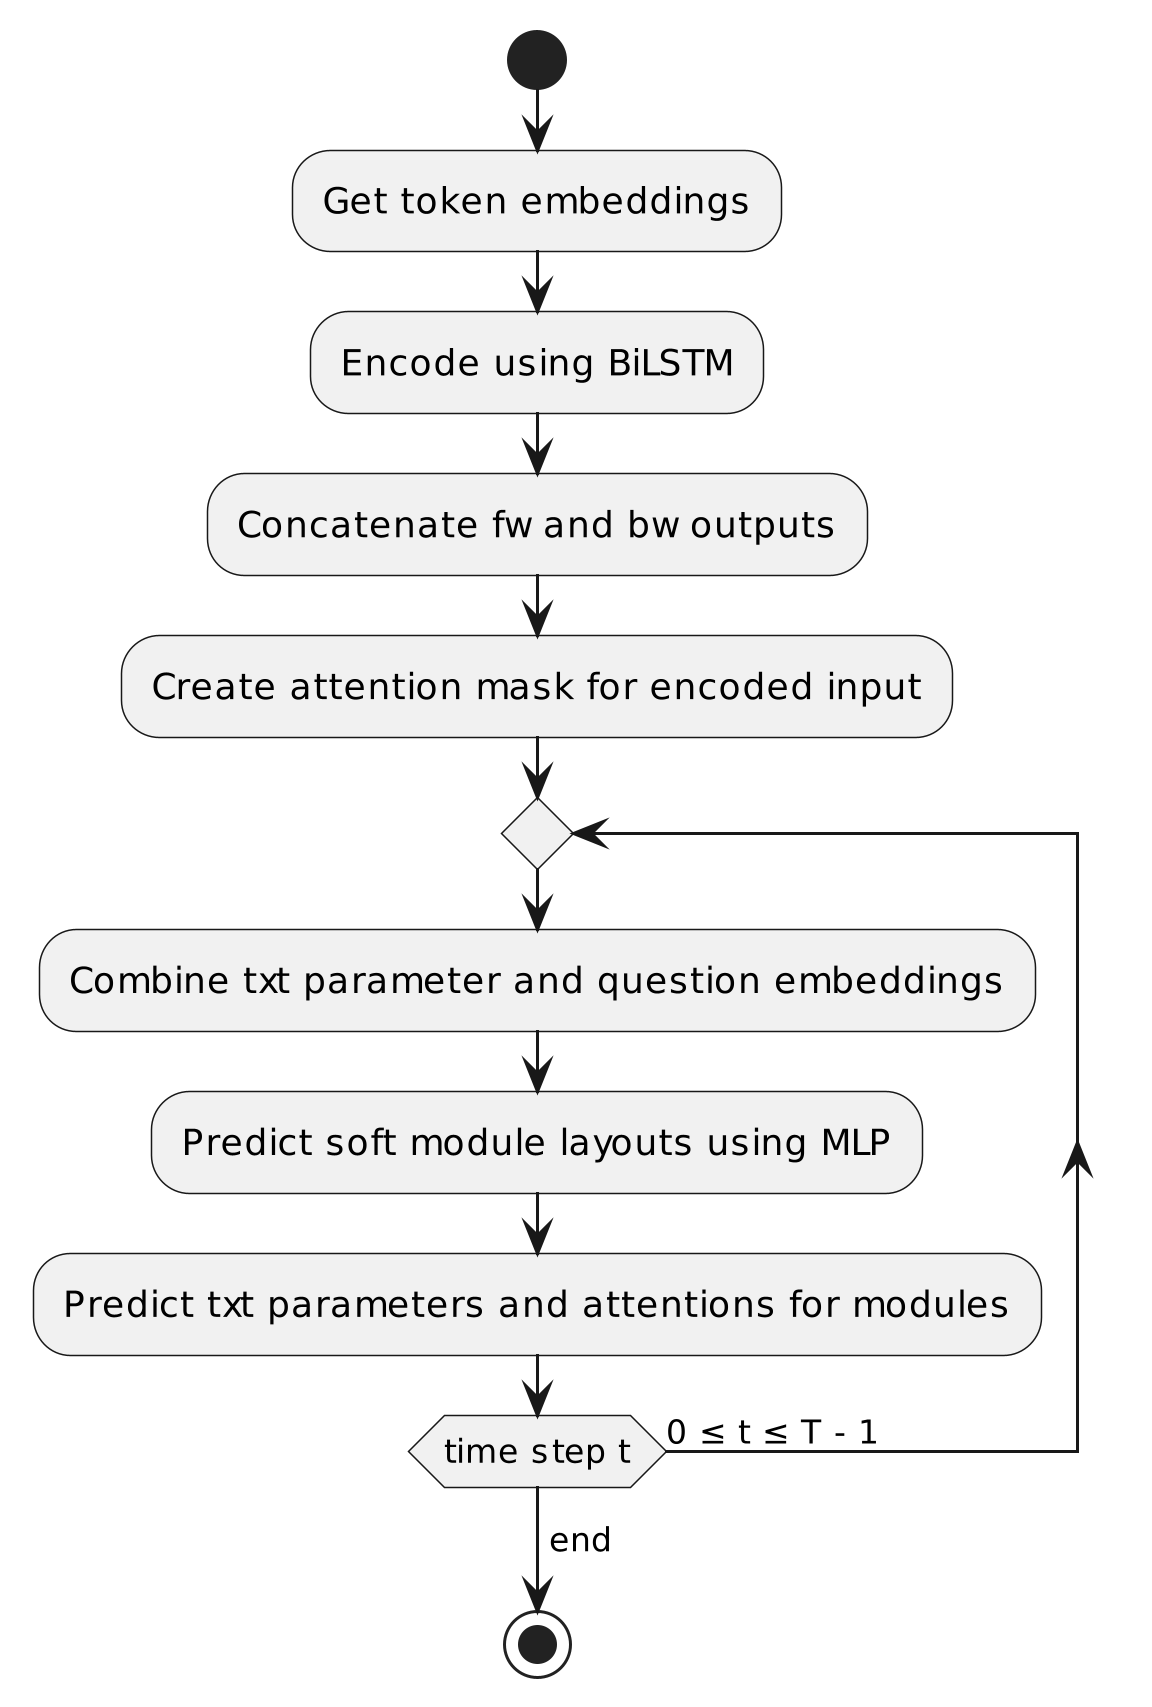
\includegraphics[width=.55\textwidth,keepaspectratio]{content/chapters/methodology/model_adaptation/figures/controller-layout-base-snmn.png}
    \captionsource(Base \gls{snmn} \gls{nas} implementation){Flow diagram of how the \gls{snmn} converts the input question to a layout.\label{fig:base_snmn_input_unit}}{Original diagram prepared for this dissertation}
\end{figure}

\begin{figure}[htbp]
    \centering
    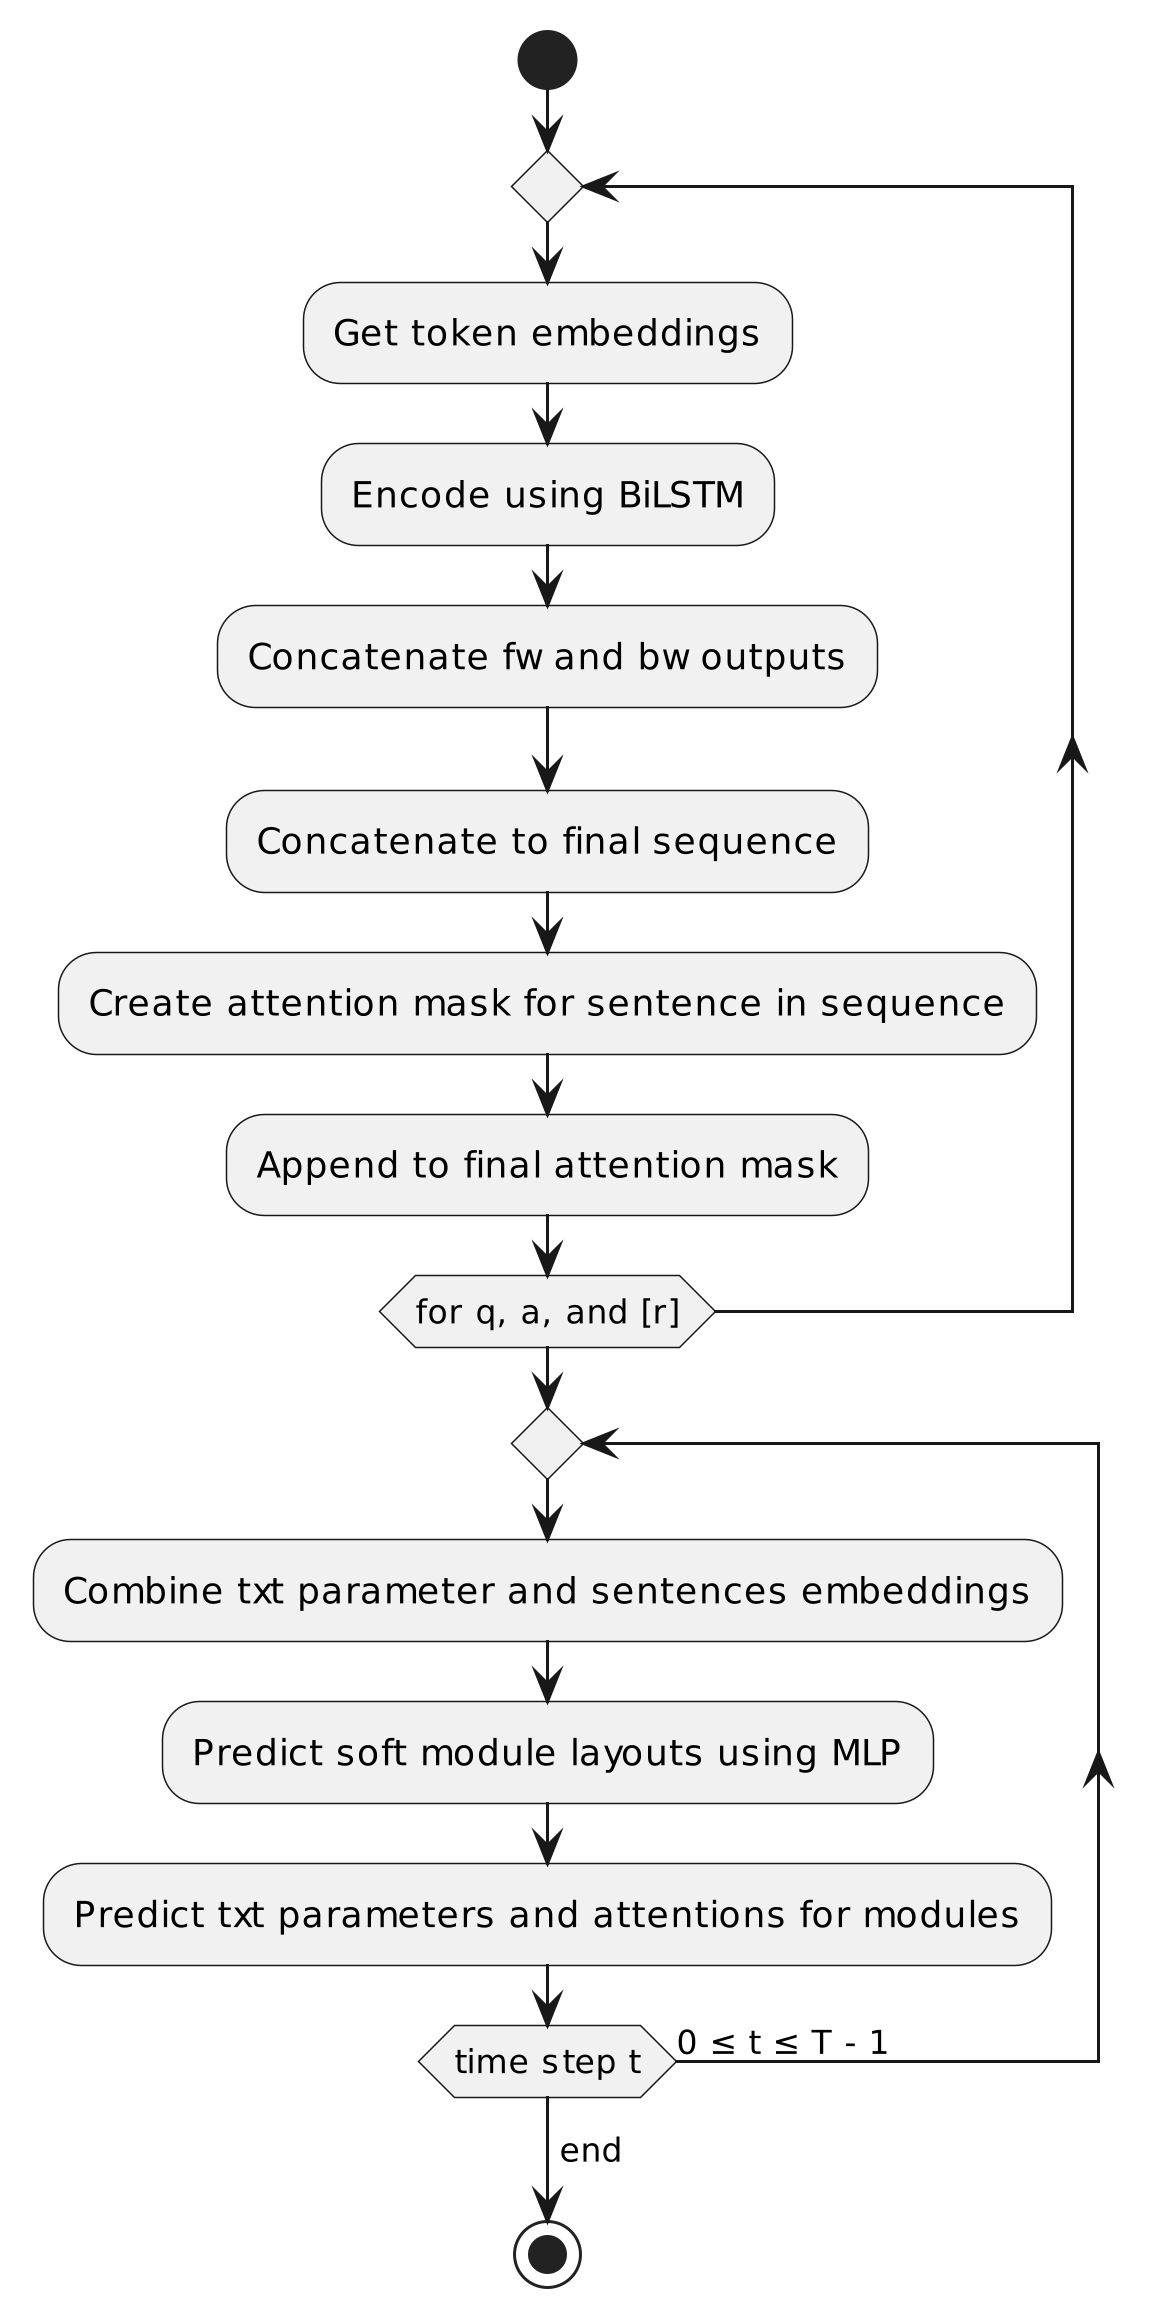
\includegraphics[width=.55\textwidth,keepaspectratio]{content/chapters/methodology/model_adaptation/figures/controller-layout-vcr-snmn.png}
    \captionsource(Modified \gls{snmn} \gls{nas} implementation){Flow diagram of how the \gls{vcr}-adapted \gls{snmn} converts the input question, answer, and rationale to a layout. Note that the rationale is only used when answering \gls{vcr} questions in QAR mode.\label{fig:vcr_snmn_input_unit}}{Original diagram prepared for this dissertation}
\end{figure}

\subsection{Output and loss function}
\label{subsec:output_and_loss_function}

Another problem arising from this question type is that it's incompatible with the original loss function of the program.
The original loss function used a softmax cross-entropy over the whole vocabulary, which is good for multilabel classification (selecting one or more correct choices) but not for multiclass classification (only one correct choice).
The new loss function uses a sigmoid cross-entropy over the prediction \glspl{logit} for each combination of question, answers, and rationales.
In other words, for each \gls{vcr} task with one question, four possible answers, and four possible rationales, the loss function will expect sixteen probability scores, with the score closest to 1 being given to the correct answer and rationale.
To form the input for the loss function, the model is run once for each input combination for the one \gls{vcr} task, a softmax vector is created from the combination of outputs, and used as input for the loss function.
